

\begin{figure}[b]
    \centering
    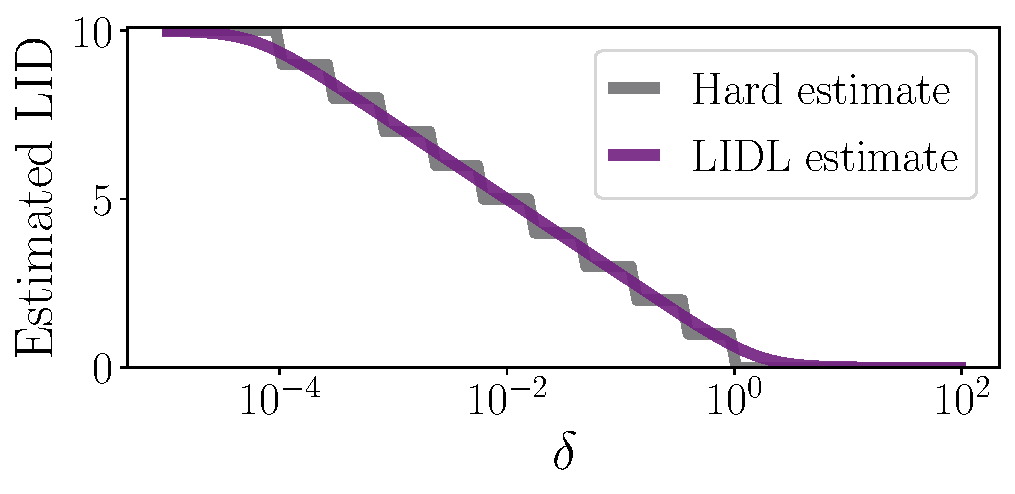
\includegraphics[width=0.4\textwidth]{images/step-delta-exp.pdf}
    \caption{LIDL and hard estimates for different values of $\delta$ for 10D non-isotripic Gaussian. Notice how LIDL ignores dimensions smaller than $\delta$, as predicted theoretically.}
    \label{fig:step-delta-exp}
\end{figure}

\subsection{Viewing $\delta$ as a scale parameter}
\label{sec:scale}



In the previous section, we glossed over the fact that we have to choose the values of $\delta$.
From Sec.~\ref{sec:core-estimate} we know that the core estimate is exact for infinitesimally small $\delta$, so the first pressure is for the $\delta$ to be small, possibly as small as the numerical precision allows. 

\begin{figure}[t]
    \centering
    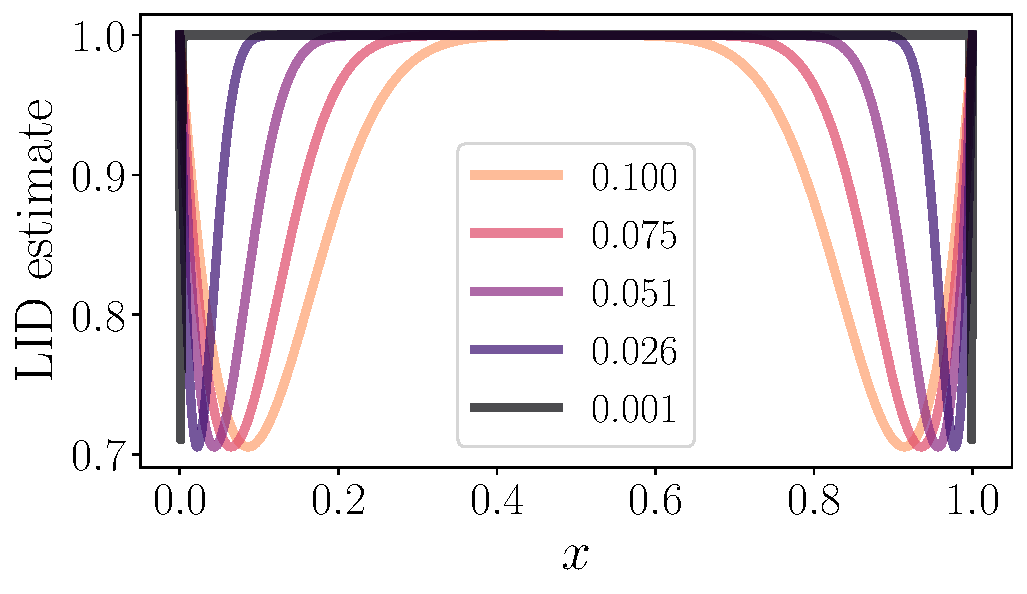
\includegraphics[width=0.4\textwidth]{images/evaluation-uniform.pdf}
    \caption{LIDL estimates for points from $\U(0,1)$ for different values of $\delta$ marked with different colors, as explained in the legend of the plot.}
    \label{fig:evaluation-uniform}
\end{figure}

However, $\delta$ can also be viewed as a length-scale parameter that allows users to choose a certain minimum `thickness' to be considered, such that dimensions `thinner' than the threshold will be ignored.
Consider an illustrative example:
suppose that the probability distribution $p_S$ is concentrated in a tubular neighborhood of another submanifold $S'$ of dimension $d'<d$. 
In this case, it can be approximated by a probability distribution $p_{S'}$ supported on $S'$.

Now, if this approximation is `good', in the sense that the thickness of the considered neighborhood is much smaller than the values of $\delta$ used, then intuitively the LIDL estimate should actually reflect the dimension $d'$ of the submanifold $S'$ instead of the true dimension $d$.

Continuing this example, 
we present the described behavior empirically. 
Let $S=\R^D$, and $p_S = \N(0, \Sigma)$, where $\Sigma$ is a diagonal matrix with entries $\sigma_1^2 \geq \sigma_2^2 \geq\dots\geq \sigma_D^2$. 
In Fig.~\ref{fig:step-delta-exp}, we plot the LIDL estimates for case $D=10$ and for $\sigma$ equally distributed on the logarithmic scale. We also plot the \emph{hard estimate} which is simply counting the number of entries in $\sigma$ that are larger than $\delta$. The LIDL estimate follows the hard estimate, and this behavior is predicted theoretically in Appendix~\ref{sec:appendix-lidl-for-normal-distribution}. 
We further investigate the role of the scale parameter in the case of imperfect density estimates in Sec.~\ref{sec:operating-range}.


As mentioned earlier, 
having an explicit length-scale parameter 
can be considered LIDL's feature as compared to other methods.
Is allows the user to easily set an operating scale such that to ignore certain amplitude of noise in the original data, e.g.\ the observation noise if we are able to estimate its magnitude apriori. 
The empirically observed rule of thumb is to take at least $\delta \gtrsim 10\sigma$, where $\sigma$ is standard deviation of the noise to be ignored. 

Setting such operating scale characteristic can be difficult in many other non-parametric algorithms that calculate statistics based on nearest neighbors. 
In those approach, there is either of the two natural scale parameters: number of nearest neighbours $k$ or radius $r$ around the point where we search for neighbours. 

When using $k$, our effective operating range depends on a combination of local density and the total number of samples used to run the algorithm. 
Using $r$ allows to set an operating range.
In this case, however, we expose ourselves to the risk of having not enough samples to estimate the local density. 
Most implementations of those methods set a default $k$.

